% *****************************************************************************************************
% ****************************              SIMPLE EXAMPLE             ********************************
% *****************************************************************************************************

% =======================================================
% =======         HEADER FOR DOCUMENT        ============
% =======================================================
    
    % *********  SPECIFIC FOR THIS BOOK  ********
    \def\ProjectAuthorLink{https://github.com/CompilandoConocimiento}
    \def\ProjectNameLink{\ProjectAuthorLink/LibroProbabilidad}    
    

    % *********   DOCUMENT ITSELF   **************
    \documentclass[12pt, fleqn]{article}                            %Type of doc and size of font and left equations
    \usepackage[margin=1.2in]{geometry}                             %Margins and Geometry pacakge
    \usepackage{ifthen}                                             %Allow simple programming using if - then
    \usepackage[hidelinks]{hyperref}                                %Allow to create hiperlinks and Fuck Firefox
    \usepackage{pdfpages}                                           %Allow us 'import' PDF's
    \hypersetup{pageanchor=false}                                   %Solve 'double page 1' warnings in build :v
    \setlength{\parindent}{0pt}                                     %Eliminate ugly indentation
    \author{Oscar Andrés Rosas}                                     %Who I am

    % *********   LANGUAJE    *****************
    \usepackage[spanish]{babel}                                     %Please allow me to type in spanish
    \usepackage[utf8]{inputenc}                                     %Lets use UFT-8
    \usepackage[T1]{fontenc}                                        %Allow for better font support
    \usepackage{textcmds}                                           %Allow us to use quoutes
    \usepackage{changepage}                                         %Allow us to use identate paragraphs
    \usepackage{anyfontsize}                                        %All the sizes for fonts wiiiii!

    % *********   MATH AND HIS STYLE  *********
    \usepackage{ntheorem, amsmath, amssymb, amsfonts}               %All fucking math, I want all!
    \usepackage{mathrsfs, mathtools, empheq}                        %All fucking math, I want all!
    \usepackage{cancel}                                             %Negate symbol
    \usepackage{centernot}                                          %Allow me to negate a symbol
    \decimalpoint                                                   %Use decimal point

    % *********   GRAPHICS AND IMAGES *********
    \usepackage{graphicx}                                           %Allow to create graphics
    \usepackage{float}                                              %For images
    \usepackage{wrapfig}                                            %Allow to create images
    \graphicspath{ {Graphics/} }                                    %Where are the images :D

    % *********   LISTS AND TABLES ***********
    \usepackage{listings, listingsutf8}                             %We will be using code here
    \usepackage[inline]{enumitem}                                   %We will need to enumarate
    \usepackage{tasks}                                              %Horizontal lists
    \usepackage{longtable}                                          %Lets make tables awesome
    \usepackage{booktabs}                                           %Lets make tables awesome
    \usepackage{tabularx}                                           %Lets make tables awesome
    \usepackage{multirow}                                           %Lets make tables awesome
    \usepackage{multicol}                                           %Create multicolumns

    % *********   REMOVE SOME ERRORS **********
    \hbadness=10000                                                 %Ignore \vbox and \hbox warings
    \hfuzz=\maxdimen\newdimen\hfuzz                                 %Ignore \vbox and \hbox warings

    % *********   HEADERS AND FOOTERS ********
    \usepackage{fancyhdr}                                           %Lets make awesome headers/footers
    \pagestyle{fancy}                                               %Lets make awesome headers/footers
    \setlength{\headheight}{16pt}                                   %Top line
    \setlength{\parskip}{0.5em}                                     %Top line
    \renewcommand{\footrulewidth}{0.5pt}                            %Bottom line


    \lhead{                                                         %Left Header
        \hyperlink{section.\arabic{section}}                        %Make a link to the current chapter
        {\normalsize{\textsc{\nouppercase{\leftmark}}}}             %And fot it put the name
    }

    \rhead{                                                         %Right Header
        \hyperlink{section.\arabic{section}.\arabic{subsection}}    %Make a link to the current chapter
            {\footnotesize{\textsc{\nouppercase{\rightmark}}}}      %And fot it put the name
    }

    \rfoot{\textsc{\small{\hyperref[sec:Index]{Ve al Índice}}}}     %This will always be a footer  

    \fancyfoot[L]{                                                  %Algoritm for a changing footer
        \ifthenelse{\isodd{\value{page}}}                           %IF ODD PAGE:
            {\href{https://SoyOscarRH.github.io/}                   %DO THIS:
                {\footnotesize                                      %Send the page
                    {\textsc{Oscar Andrés Rosas}}}}                 %Send the page
            {\href{https://compilandoconocimiento.com}              %ELSE DO THIS: 
                {\footnotesize                                      %Send the author
                    {\textsc{Compilando Conocimiento}}}}            %Send the author
    }
    
    
% =======================================================
% ===================   COMMANDS    =====================
% =======================================================

    % =========================================
    % =======   NEW ENVIRONMENTS   ============
    % =========================================
    \newenvironment{Indentation}[1][0.75em]                         %Use: \begin{Inde...}[Num]...\end{Inde...}
        {\begin{adjustwidth}{#1}{}}                                 %If you dont put nothing i will use 0.75 em
        {\end{adjustwidth}}                                         %This indentate a paragraph
    
    \newenvironment{SmallIndentation}[1][0.75em]                    %Use: The same that we upper one, just 
        {\begin{adjustwidth}{#1}{}\begin{footnotesize}}             %footnotesize size of letter by default
        {\end{footnotesize}\end{adjustwidth}}                       %that's it
    
    \def \Eq {equation}                                             %Stupid Visual studio error
    \newenvironment{MultiLineEquation}[1]                           %Use: To create MultiLine equations
        {\begin{\Eq}\begin{alignedat}{#1}}                          %Use: \begin{Multi..}{Num. de Columnas}
        {\end{alignedat}\end{\Eq}}                                  %And.. that's it!
    
    \newenvironment{MultiLineEquation*}[1]                          %Use: To create MultiLine equations
        {\begin{\Eq*}\begin{alignedat}{#1}}                         %Use: \begin{Multi..}{Num. de Columnas}
        {\end{alignedat}\end{\Eq*}}                                 %And.. that's it!

    \newenvironment{LargeEq} {\begingroup \Large}{\endgroup}        %Make eq bigger
    \newenvironment{HugeEq} {\begingroup \Huge}{\endgroup}          %Make eq bigger!
    

    % =========================================
    % == GENERAL TEXT & SYMBOLS ENVIRONMENTS ==
    % =========================================
    
    % =====  TEXT  ======================
    \newcommand \Quote              {\qq}                           %Use: \Quote to use quotes
    \newcommand \Over               {\overline}                     %Use: \Bar to use just for short
    \newcommand \ForceNewLine       {$\Space$\\}                    %Use it in theorems for example
    \newcommand \ForceColumnBreak   {\vfill\null\columnbreak}       %Use only in multicols

    % =====  SPACES  ====================
    \DeclareMathOperator \Space     {\quad}                         %Use: \Space for a cool mega space
    \DeclareMathOperator \MegaSpace {\quad \quad}                   %Use: \MegaSpace for a cool mega mega space
    \DeclareMathOperator \MiniSpace {\;}                            %Use: \Space for a cool mini space
    
    % =====  MATH TEXT  =================
    \newcommand \Such           {\MiniSpace | \MiniSpace}           %Use: \Such like in sets
    \newcommand \Also           {\MiniSpace \text{y} \MiniSpace}    %Use: \Also so it's look cool
    \newcommand \Remember[1]    {\Space\text{\scriptsize{#1}}}      %Use: \Remember so it's look cool
    
    % =====  THEOREMS: IN SPANISH :0  ===
    \newtheorem{Theorem}        {Teorema}[section]                  %Use: \begin{Theorem}[Name]\label{Nombre}...
    \newtheorem{Corollary}      {Colorario}[Theorem]                %Use: \begin{Corollary}[Name]\label{Nombre}...
    \newtheorem{Lemma}[Theorem] {Lemma}                             %Use: \begin{Lemma}[Name]\label{Nombre}...
    \newtheorem{Definition}     {Definición}[section]               %Use: \begin{Definition}[Name]\label{Nombre}...
    \theoremstyle{break}                                            %THEOREMS START 1 SPACE AFTER Fuck!

    % =====  LOGIC  =====================
    \newcommand \lIff    {\leftrightarrow}                          %Use: \lIff for logic iff
    \newcommand \lEqual  {\MiniSpace \Leftrightarrow \MiniSpace}    %Use: \lEqual for a logic double arrow
    \newcommand \lInfire {\MiniSpace \Rightarrow \MiniSpace}        %Use: \lInfire for a logic infire
    \newcommand \lLongTo {\longrightarrow}                          %Use: \lLongTo for a long arrow
    \newcommand \lAnd    {\land}                                    %Use: \lAnd ^
    \newcommand \lOr     {\lor}                                     %Use: \lOr or symbol
    \newcommand \lNot    {\neg}                                     %Use: \lNot for negation

    % =====  FAMOUS SETS  ===============
    \DeclareMathOperator \Naturals     {\mathbb{N}}                 %Use: \Naturals por Notation
    \DeclareMathOperator \Primes       {\mathbb{P}}                 %Use: \Primes por Notation
    \DeclareMathOperator \Integers     {\mathbb{Z}}                 %Use: \Integers por Notation
    \DeclareMathOperator \Racionals    {\mathbb{Q}}                 %Use: \Racionals por Notation
    \DeclareMathOperator \Reals        {\mathbb{R}}                 %Use: \Reals por Notation
    \DeclareMathOperator \Complexs     {\mathbb{C}}                 %Use: \Complex por Notation
    \DeclareMathOperator \GenericField {\mathbb{F}}                 %Use: \GenericField por Notation
    \DeclareMathOperator \VectorSet    {\mathbb{V}}                 %Use: \VectorSet por Notation
    \DeclareMathOperator \SubVectorSet {\mathbb{W}}                 %Use: \SubVectorSet por Notation
    \DeclareMathOperator \Polynomials  {\mathbb{P}}                 %Use: \Polynomials por Notation
    \DeclareMathOperator \VectorSpace  {\VectorSet_{\GenericField}} %Use: \VectorSpace por Notation
    \DeclareMathOperator \LinealTransformation {\mathcal{T}}        %Use: \LinealTransformation for a cool T
    \DeclareMathOperator \LinTrans      {\mathcal{T}}               %Use: \LinTrans for a cool T
    \DeclareMathOperator \Laplace       {\mathcal{L}}               %Use: \LinTrans for a cool T

    % =====  CONTAINERS   ===============
    \newcommand{\Set}[1]            {\left\{ \; #1 \; \right\}}     %Use: \Set {Info} for INTELLIGENT space 
    \newcommand{\bigSet}[1]         {\big\{  \; #1 \; \big\}}       %Use: \bigSet  {Info} for space 
    \newcommand{\BigSet}[1]         {\Big\{  \; #1 \; \Big\}}       %Use: \BigSet  {Info} for space 
    \newcommand{\biggSet}[1]        {\bigg\{ \; #1 \; \bigg\}}      %Use: \biggSet {Info} for space 
    \newcommand{\BiggSet}[1]        {\Bigg\{ \; #1 \; \Bigg\}}      %Use: \BiggSet {Info} for space 
        
    \newcommand{\Wrap}[1]           {\left( #1 \right)}             %Use: \Wrap {Info} for INTELLIGENT space
    \newcommand{\bigWrap}[1]        {\big( \; #1 \; \big)}          %Use: \bigBrackets  {Info} for space 
    \newcommand{\BigWrap}[1]        {\Big( \; #1 \; \Big)}          %Use: \BigBrackets  {Info} for space 
    \newcommand{\biggWrap}[1]       {\bigg( \; #1 \; \bigg)}        %Use: \biggBrackets {Info} for space 
    \newcommand{\BiggWrap}[1]       {\Bigg( \; #1 \; \Bigg)}        %Use: \BiggBrackets {Info} for space 

    \newcommand{\Brackets}[1]       {\left[ #1 \right]}             %Use: \Brackets {Info} for INTELLIGENT space
    \newcommand{\bigBrackets}[1]    {\big[ \; #1 \; \big]}          %Use: \bigBrackets  {Info} for space 
    \newcommand{\BigBrackets}[1]    {\Big[ \; #1 \; \Big]}          %Use: \BigBrackets  {Info} for space 
    \newcommand{\biggBrackets}[1]   {\bigg[ \; #1 \; \bigg]}        %Use: \biggBrackets {Info} for space 
    \newcommand{\BiggBrackets}[1]   {\Bigg[ \; #1 \; \Bigg]}        %Use: \BiggBrackets {Info} for space 

    \newcommand{\Generate}[1]   {\left\langle #1 \right\rangle}     %Use: \Generate {Info} <>
    \newcommand{\Floor}[1]      {\left \lfloor #1 \right \rfloor}   %Use: \Floor {Info} for floor 
    \newcommand{\Ceil}[1]       {\left \lceil #1 \right \rceil }    %Use: \Ceil {Info} for ceil
    
    % =====  BETTERS MATH COMMANDS   =====
    \newcommand{\pfrac}[2]      {\Wrap{\dfrac{#1}{#2}}}             %Use: Put fractions in parentesis

    % =========================================
    % ====   LINEAL ALGEBRA & VECTORS    ======
    % =========================================

    % ===== UNIT VECTORS  ================
    \newcommand{\hati}      {\hat{\imath}}                           %Use: \hati for unit vector    
    \newcommand{\hatj}      {\hat{\jmath}}                           %Use: \hatj for unit vector    
    \newcommand{\hatk}      {\hat{k}}                                %Use: \hatk for unit vector

    % ===== MAGNITUDE  ===================
    \newcommand{\abs}[1]    {\left\lvert #1 \right\lvert}           %Use: \abs{expression} for |x|
    \newcommand{\Abs}[1]    {\left\lVert #1 \right\lVert}           %Use: \Abs{expression} for ||x||
    \newcommand{\Mag}[1]    {\left| #1 \right|}                     %Use: \Mag {Info} 
    
    \newcommand{\bVec}[1]   {\mathbf{#1}}                           %Use for bold type of vector
    \newcommand{\lVec}[1]   {\overrightarrow{#1}}                   %Use for a long arrow over a vector
    \newcommand{\uVec}[1]   {\mathbf{\hat{#1}}}                     %Use: Unitary Vector Example: $\uVec{i}

    % ===== FN LINEAL TRANSFORMATION  ====
    \newcommand{\FnLinTrans}[1]{\mathcal{T}\Wrap{#1}}               %Use: \FnLinTrans for a cool T
    \newcommand{\VecLinTrans}[1]{\mathcal{T}\pVector{#1}}           %Use: \LinTrans for a cool T
    \newcommand{\FnLinealTransformation}[1]{\mathcal{T}\Wrap{#1}}   %Use: \FnLinealTransformation

    % ===== ALL FOR DOT PRODUCT  =========
    \makeatletter                                                   %WTF! IS THIS
    \newcommand*\dotP{\mathpalette\dotP@{.5}}                       %Use: \dotP for dot product
    \newcommand*\dotP@[2] {\mathbin {                               %WTF! IS THIS            
        \vcenter{\hbox{\scalebox{#2}{$\m@th#1\bullet$}}}}           %WTF! IS THIS
    }                                                               %WTF! IS THIS
    \makeatother                                                    %WTF! IS THIS

    % === WRAPPERS FOR COLUMN VECTOR ===
    \newcommand{\pVector}[1]                                        %Use: \pVector {Matrix Notation} use parentesis
        { \ensuremath{\begin{pmatrix}#1\end{pmatrix}} }             %Example: \pVector{a\\b\\c} or \pVector{a&b&c} 
    \newcommand{\lVector}[1]                                        %Use: \lVector {Matrix Notation} use a abs 
        { \ensuremath{\begin{vmatrix}#1\end{vmatrix}} }             %Example: \lVector{a\\b\\c} or \lVector{a&b&c} 
    \newcommand{\bVector}[1]                                        %Use: \bVector {Matrix Notation} use a brackets 
        { \ensuremath{\begin{bmatrix}#1\end{bmatrix}} }             %Example: \bVector{a\\b\\c} or \bVector{a&b&c} 
    \newcommand{\Vector}[1]                                         %Use: \Vector {Matrix Notation} no parentesis
        { \ensuremath{\begin{matrix}#1\end{matrix}} }               %Example: \Vector{a\\b\\c} or \Vector{a&b&c}

    % === MAKE MATRIX BETTER  =========
    \makeatletter                                                   %Example: \begin{matrix}[cc|c]
    \renewcommand*\env@matrix[1][*\c@MaxMatrixCols c] {             %WTF! IS THIS
        \hskip -\arraycolsep                                        %WTF! IS THIS
        \let\@ifnextchar\new@ifnextchar                             %WTF! IS THIS
        \array{#1}                                                  %WTF! IS THIS
    }                                                               %WTF! IS THIS
    \makeatother                                                    %WTF! IS THIS

    % =========================================
    % =======   FAMOUS FUNCTIONS   ============
    % =========================================

    % == TRIGONOMETRIC FUNCTIONS  ====
    \newcommand{\Cos}[1] {\cos\Wrap{#1}}                            %Simple wrappers
    \newcommand{\Sin}[1] {\sin\Wrap{#1}}                            %Simple wrappers
    \newcommand{\Tan}[1] {tan\Wrap{#1}}                             %Simple wrappers
    
    \newcommand{\Sec}[1] {sec\Wrap{#1}}                             %Simple wrappers
    \newcommand{\Csc}[1] {csc\Wrap{#1}}                             %Simple wrappers
    \newcommand{\Cot}[1] {cot\Wrap{#1}}                             %Simple wrappers

    % === COMPLEX ANALYSIS TRIG ======
    \newcommand \Cis[1]  {\Cos{#1} + i \Sin{#1}}                    %Use: \Cis for cos(x) + i sin(x)
    \newcommand \pCis[1] {\Wrap{\Cis{#1}}}                          %Use: \pCis for the same with parantesis
    \newcommand \bCis[1] {\Brackets{\Cis{#1}}}                      %Use: \bCis for the same with Brackets


    % =========================================
    % ===========     CALCULUS     ============
    % =========================================

    % ====== TRANSFORMS =============
    \newcommand{\FourierT}[1]   {\mathscr{F} \left\{ #1 \right\} }  %Use: \FourierT {Funtion}
    \newcommand{\InvFourierT}[1]{\mathscr{F}^{-1}\left\{#1\right\}} %Use: \InvFourierT {Funtion}

    % ====== DERIVATIVES ============
    \newcommand \MiniDerivate[1][x]   {\dfrac{d}{d #1}}             %Use: \MiniDerivate[var] for simple use [var]
    \newcommand \Derivate[2]          {\dfrac{d \; #1}{d #2}}       %Use: \Derivate [f(x)][x]
    \newcommand \MiniUpperDerivate[2] {\dfrac{d^{#2}}{d#1^{#2}}}    %Mini Derivate High Orden Derivate -- [x][pow]
    \newcommand \UpperDerivate[3] {\dfrac{d^{#3} \; #1}{d#2^{#3}}}  %Complete High Orden Derivate -- [f(x)][x][pow]
    
    \newcommand \MiniPartial[1][x] {\dfrac{\partial}{\partial #1}}  %Use: \MiniDerivate for simple use [var]
    \newcommand \Partial[2] {\dfrac{\partial \; #1}{\partial #2}}   %Complete Partial Derivate -- [f(x)][x]
    \newcommand \MiniUpperPartial[2]                                %Mini Derivate High Orden Derivate -- [x][pow] 
        {\dfrac{\partial^{#2}}{\partial #1^{#2}}}                   %Mini Derivate High Orden Derivate
    \newcommand \UpperPartial[3]                                    %Complete High Orden Derivate -- [f(x)][x][pow]
        {\dfrac{\partial^{#3} \; #1}{\partial#2^{#3}}}              %Use: \UpperDerivate for simple use

    \DeclareMathOperator \Evaluate  {\Big|}                         %Use: \Evaluate por Notation

    % ====== INTEGRALS ============
    \newcommand{\inftyInt} {\int_{-\infty}^{\infty}}                %Use: \inftyInt for simple integrants
      

% =======================================================
% ===========      COLOR: MATERIAL DESIGN     ===========
% =======================================================

    % =====  COLORS ==================
    \definecolor{RedMD}{HTML}{F44336}                               %Use: Color :D        
    \definecolor{Red100MD}{HTML}{FFCDD2}                            %Use: Color :D        
    \definecolor{Red200MD}{HTML}{EF9A9A}                            %Use: Color :D        
    \definecolor{Red300MD}{HTML}{E57373}                            %Use: Color :D        
    \definecolor{Red700MD}{HTML}{D32F2F}                            %Use: Color :D 

    \definecolor{PurpleMD}{HTML}{9C27B0}                            %Use: Color :D        
    \definecolor{Purple100MD}{HTML}{E1BEE7}                         %Use: Color :D        
    \definecolor{Purple200MD}{HTML}{EF9A9A}                         %Use: Color :D        
    \definecolor{Purple300MD}{HTML}{BA68C8}                         %Use: Color :D        
    \definecolor{Purple700MD}{HTML}{7B1FA2}                         %Use: Color :D 

    \definecolor{IndigoMD}{HTML}{3F51B5}                            %Use: Color :D        
    \definecolor{Indigo100MD}{HTML}{C5CAE9}                         %Use: Color :D        
    \definecolor{Indigo200MD}{HTML}{9FA8DA}                         %Use: Color :D        
    \definecolor{Indigo300MD}{HTML}{7986CB}                         %Use: Color :D        
    \definecolor{Indigo700MD}{HTML}{303F9F}                         %Use: Color :D 

    \definecolor{BlueMD}{HTML}{2196F3}                              %Use: Color :D        
    \definecolor{Blue100MD}{HTML}{BBDEFB}                           %Use: Color :D        
    \definecolor{Blue200MD}{HTML}{90CAF9}                           %Use: Color :D        
    \definecolor{Blue300MD}{HTML}{64B5F6}                           %Use: Color :D        
    \definecolor{Blue700MD}{HTML}{1976D2}                           %Use: Color :D        
    \definecolor{Blue900MD}{HTML}{0D47A1}                           %Use: Color :D  

    \definecolor{CyanMD}{HTML}{00BCD4}                              %Use: Color :D        
    \definecolor{Cyan100MD}{HTML}{B2EBF2}                           %Use: Color :D        
    \definecolor{Cyan200MD}{HTML}{80DEEA}                           %Use: Color :D        
    \definecolor{Cyan300MD}{HTML}{4DD0E1}                           %Use: Color :D        
    \definecolor{Cyan700MD}{HTML}{0097A7}                           %Use: Color :D        
    \definecolor{Cyan900MD}{HTML}{006064}                           %Use: Color :D 

    \definecolor{TealMD}{HTML}{009688}                              %Use: Color :D        
    \definecolor{Teal100MD}{HTML}{B2DFDB}                           %Use: Color :D        
    \definecolor{Teal200MD}{HTML}{80CBC4}                           %Use: Color :D        
    \definecolor{Teal300MD}{HTML}{4DB6AC}                           %Use: Color :D        
    \definecolor{Teal700MD}{HTML}{00796B}                           %Use: Color :D        
    \definecolor{Teal900MD}{HTML}{004D40}                           %Use: Color :D 

    \definecolor{GreenMD}{HTML}{4CAF50}                             %Use: Color :D        
    \definecolor{Green100MD}{HTML}{C8E6C9}                          %Use: Color :D        
    \definecolor{Green200MD}{HTML}{A5D6A7}                          %Use: Color :D        
    \definecolor{Green300MD}{HTML}{81C784}                          %Use: Color :D        
    \definecolor{Green700MD}{HTML}{388E3C}                          %Use: Color :D        
    \definecolor{Green900MD}{HTML}{1B5E20}                          %Use: Color :D

    \definecolor{AmberMD}{HTML}{FFC107}                             %Use: Color :D        
    \definecolor{Amber100MD}{HTML}{FFECB3}                          %Use: Color :D        
    \definecolor{Amber200MD}{HTML}{FFE082}                          %Use: Color :D        
    \definecolor{Amber300MD}{HTML}{FFD54F}                          %Use: Color :D        
    \definecolor{Amber700MD}{HTML}{FFA000}                          %Use: Color :D        
    \definecolor{Amber900MD}{HTML}{FF6F00}                          %Use: Color :D

    \definecolor{BlueGreyMD}{HTML}{607D8B}                          %Use: Color :D        
    \definecolor{BlueGrey100MD}{HTML}{CFD8DC}                       %Use: Color :D        
    \definecolor{BlueGrey200MD}{HTML}{B0BEC5}                       %Use: Color :D        
    \definecolor{BlueGrey300MD}{HTML}{90A4AE}                       %Use: Color :D        
    \definecolor{BlueGrey700MD}{HTML}{455A64}                       %Use: Color :D        
    \definecolor{BlueGrey900MD}{HTML}{263238}                       %Use: Color :D        

    \definecolor{DeepPurpleMD}{HTML}{673AB7}                        %Use: Color :D

    % =====  ENVIRONMENT ==============
    \newcommand{\Color}[2]{\textcolor{#1}{#2}}                      %Simple color environment
    \newenvironment{ColorText}[1]                                   %Use: \begin{ColorText}
        { \leavevmode\color{#1}\ignorespaces }                      %That's is!


% =======================================================
% ===========           CODE EDITING          ===========
% =======================================================

    % =====  CODE EDITOR =============
    \lstdefinestyle{CompilandoStyle} {                              %This is Code Style
        backgroundcolor     = \color{BlueGrey900MD},                %Background Color  
        basicstyle          = \tiny\color{white},                   %Style of text
        commentstyle        = \color{BlueGrey200MD},                %Comment style
        stringstyle         = \color{Green300MD},                   %String style
        keywordstyle        = \color{Blue300MD},                    %keywords style
        numberstyle         = \tiny\color{TealMD},                  %Size of a number
        frame               = shadowbox,                            %Adds a frame around the code
        breakatwhitespace   = true,                                 %Style   
        breaklines          = true,                                 %Style   
        showstringspaces    = false,                                %Hate those spaces                  
        breaklines          = true,                                 %Style                   
        keepspaces          = true,                                 %Style                   
        numbers             = left,                                 %Style                   
        numbersep           = 10pt,                                 %Style 
        xleftmargin         = \parindent,                           %Style 
        tabsize             = 4,                                    %Style
        inputencoding       = utf8/latin1                           %Allow me to use special chars
    }

    % =====  CODE EDITOR =============
    \lstdefinestyle{CompilandoStylePurity} {                        %This is Code Style
        backgroundcolor     = \color{white},                        %Background Color  
        basicstyle          = \tiny\color{BlueGrey900MD},           %Style of text
        commentstyle        = \color{Green300MD},                   %Comment style
        stringstyle         = \color{Teal700MD},                    %String style
        keywordstyle        = \color{Blue700MD},                    %keywords style
        numberstyle         = \tiny\color{TealMD},                  %Size of a number
        frame               = none,                                 %Adds a frame around the code
        breakatwhitespace   = true,                                 %Style   
        breaklines          = true,                                 %Style   
        showstringspaces    = false,                                %Hate those spaces                  
        breaklines          = true,                                 %Style                   
        keepspaces          = true,                                 %Style                   
        numbers             = left,                                 %Style                   
        numbersep           = 11pt,                                 %Style 
        xleftmargin         = \parindent,                           %Style 
        tabsize             = 4,                                    %Style
        inputencoding       = utf8/latin1                           %Allow me to use special chars
    }
 
    \lstset{style = CompilandoStyle}                                %Use this style
    
    
    
    

% =====================================================
% ============        COVER PAGE       ================
% =====================================================
\begin{document}
\begin{titlepage}
    
    % ============ TITLE PAGE STYLE  ================
    \definecolor{TitlePageColor}{cmyk}{1,.60,0,.40}                 %Simple colors
    \definecolor{ColorSubtext}{cmyk}{1,.50,0,.10}                   %Simple colors
    \newgeometry{left=0.25\textwidth}                               %Defines an Offset
    \pagecolor{TitlePageColor}                                      %Make it this Color to page
    \color{white}                                                   %General things should be white

    % ===== MAKE SOME SPACE =========
    \vspace                                                         %Give some space
    \baselineskip                                                   %But we need this to up command

    % ============ NAME OF THE PROJECT  ============
    \makebox[0pt][l]{\rule{1.3\textwidth}{3pt}}                     %Make a cool line
    
    \href{https://compilandoconocimiento.com}                       %Link to project
    {\textbf{\textsc{\Huge Estructuras Discretas}}}\\[2.7cm]      %Name of project   

    % ============ NAME OF THE BOOK  ===============
    \href{\ProjectNameLink}                                         %Link to Author
    {\fontsize{45}{52}\selectfont \textbf{Tarea 5}}\\[0.5cm]        %Name of the book
    \textcolor{ColorSubtext}{\textsc{\Huge Grafos / Gráficas}}      %Name of the general theme
    
    \vfill                                                          %Fill the space
    
    % ============ NAME OF THE AUTHOR  =============
    \href{\ProjectAuthorLink}                                       %Link to Author
    {\LARGE \textsf{Oscar Andrés Rosas Hernandez}}                  %Author

    % ===== MAKE SOME SPACE =========
    \vspace                                                         %Give some space
    \baselineskip                                                   %But we need this to up command
    
    {\large \textsf{Diciembre 2018}}                                %Date

\end{titlepage}


% =====================================================
% ==========      RESTORE TO DOCUMENT      ============
% =====================================================
\restoregeometry                                                    %Restores the geometry
\nopagecolor                                                        %Use to restore the color to white




% =====================================================
% ========                INDICE              =========
% =====================================================
\tableofcontents{}
\label{sec:Index}

\clearpage

% ===============================================
% ========              1                 =======
% ===============================================
\clearpage
\section{Pregunta 2}

    Prueba que hay 11 gráficas no isomorfas con 4 vértices.

    % ======== DEMOSTRACION ========
    \begin{SmallIndentation}[1em]
        \textbf{Demostración}:

            Vamos a llamar a los vértices $1, 2, 3, 4$, ahora vamos a iterar sobre las aristas:
            Supongamos que tenemos:
            \begin{itemize}
                \item Con $0$ aristas solo podemos tener un grafo, en el que todos estan desconectados.
                \item Con $1$ aristas solo podemos tener un grafo \\
                    \begin{itemize}
                        \item Por ejemplo:$(1,2)$, $(2, 3)$, $(3, 4)$
                    \end{itemize}
                    
                \item Con $2$ aristas solo podemos tener dos grafos \\
                    \begin{itemize}
                        \item $(1,2)$ y $(2,3)$
                        \item $(1,2)$ y $(3,4)$
                    \end{itemize}
                
                \item Con $3$ aristas solo podemos tener 3 grafos \\
                    \begin{itemize}
                        \item $(1,2), (2,4)$ y $(2,3)$
                        \item $(1,2), (2,3)$ y $(1,3)$
                        \item $(1,2), (2,3)$ y $(3,4)$
                    \end{itemize}

                \item Con $4$ aristas solo podemos tener dos grafos \\
                    \begin{itemize}
                        \item $(1,2), (2,3), (3,4)$ y $(1,4)$
                        \item $(1,2), (2,3), (1,3)$ y $(2,4)$
                    \end{itemize}

                \item Con $5$ aristas solo podemos tener 1 grafo \\
                    \begin{itemize}
                        \item $(1,2), (2,3), (3,4), (1,4)$ y $(1,3)$
                    \end{itemize}

                \item Con $6$ aristas solo podemos tener 1 grafo \\
                    \begin{itemize}
                        \item $(1,2), (2,3), (3,4), (1,4), (1,3)$ y $(2,4)$
                    \end{itemize}
            \end{itemize}

            Recuerda que un grafo completo tendrá $\frac{n(n-1)}{2}$ es decir $6$ aristas, por lo
            tanto no puede un grafo tener más aristas.

            Ahora si sumamos: $1+1+2+3+2+1+1 = 11$
        

    \end{SmallIndentation}



% ===============================================
% ========              4                 =======
% ===============================================
\clearpage
\section{Pregunta 4}

    Muestra que las siguientes gráficas no simples no son isomorfas.

    Conste que dice muestra y no prueba en si, así que esto será mas bien un bosquejo.

    Primero, si es que fueran isomorfas entonces tendría que existir un mapeo entre vértices
    nos daría como resultado dos grafos iguales.

    Ahora, enfoquemos en ese nodo que va hacia si mismo.
    Creo que es obvio que el hecho de que existe un solo de este tipo de vértices solo nos deja un mapeo que parece
    ser valido:

    \begin{figure}[h]
        \centering
        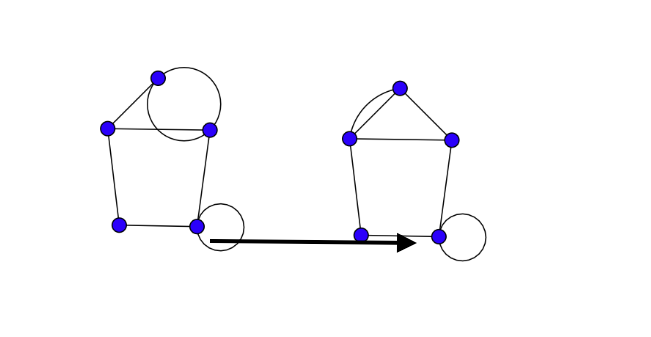
\includegraphics[width=0.35\textwidth]{Question41}
    \end{figure}

    Ahora veamos porque este mapeo esta mal, veamos los vértices adjacentes a ese nodo.
    Ahi es donde notamos una diferencia, en los grados de dichos vértices, por lo tanto ese mapeo tampoco puede ser valido
    \begin{figure}[h]
        \centering
        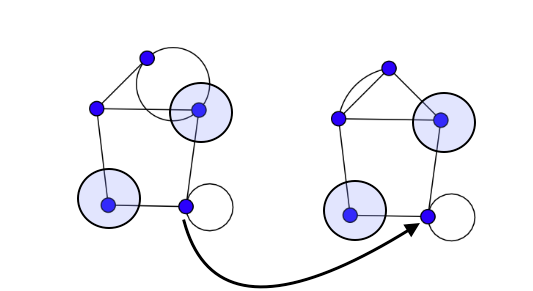
\includegraphics[width=0.35\textwidth]{Question42}
    \end{figure}

    Por lo tanto no son isomorfas
    



    % ===============================================
    % ========              6                 =======
    % ===============================================
    \clearpage
    \section{Pregunta 6}

        % ======== DEMOSTRACION ========
        \begin{SmallIndentation}[1em]
            \textbf{Demostración}:
        
            Basta con saber que si se tienen $n$ vértices entonces se tendrá a lo máximo $\dfrac{n (n-1)}{2}$ aristas.

            Usando un sencillo codigo en Python podemos para $n$ vértices cuantas aristas máximas pueden tener:

            \begin{lstlisting}[language=python, gobble=12]
                for vertices in range(1, 12):
                    print (f"Vertices {vertices}: ")
                    print (int((vertices * (vertices - 1)) / 2 ))
            \end{lstlisting}

            Así vemos que si tienes 10 vertices entonces puedes tener máximo 45 aristas y seguir siendo un grafo simple,
            ahora, si tienes 11 vertices entonces puedes tener hasta 55 aristas, por lo tanto la respuesta es 11.

        \end{SmallIndentation}


    % ===============================================
    % ========              7                 =======
    % ===============================================
    \section{Pregunta 7}

        % ======== DEMOSTRACION ========
        \begin{SmallIndentation}[1em]
            \textbf{Demostración}:
        
            Basta con recordar un teorema que pronto demostraré que dice que la suma del los grados de todos los vertices
            de un grafo es el doble de las aristas del mismo, por lo tanto:

            \begin{MultiLineEquation*}{3}
                aristas = \dfrac{4+3+3+2+2}{2} = 7
            \end{MultiLineEquation*}
        
        \end{SmallIndentation}


    % ===============================================
    % ========              9                 =======
    % ===============================================
    \clearpage
    \section{Pregunta 9}

    % ======== DEMOSTRACION ========
    \begin{SmallIndentation}[1em]
        \textbf{Demostración}:
    
        Esta esta sencilla, lo que en escencia se esta haciendo es preguntar si se puede hacer un nodo que tiene
        6 vertices y 9 aristas tal que el grado de cualquier nodo es 3. Y claro que es posible, por el mismo argumento
        que en la anterior pregunta, si sumo 6 veces 3 entonces tengo 18 que entre dos nos da 9, así que todo perfecto.

        Ahora, la idea es saber si es unica, lo que hice fue buscar todas las graficas de 6 vertices y 9 aristas y ver si
        habia dos que tuviera grado 3 en todos sus vértices.
        Y la respuesta es ... no.

        \begin{figure}[h]
            \centering
            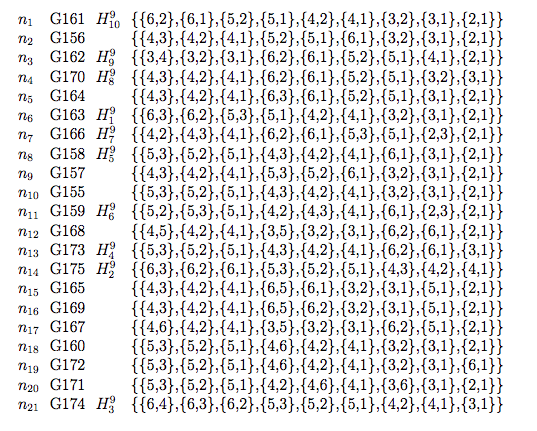
\includegraphics[width=0.35\textwidth]{Question91}
        \end{figure}

        \begin{figure}[h]
            \centering
            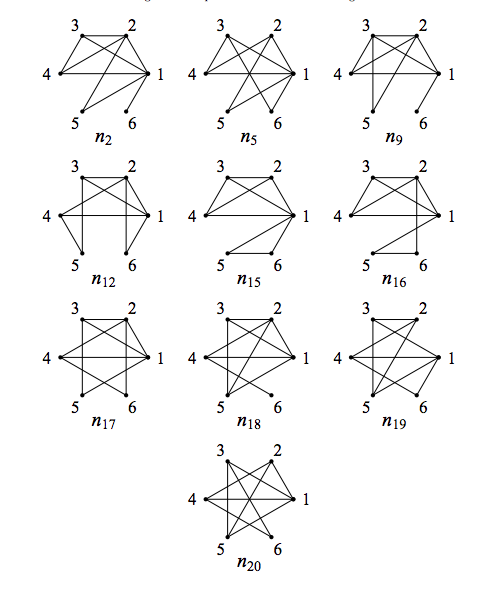
\includegraphics[width=0.35\textwidth]{Question92}
        \end{figure}
    
    \end{SmallIndentation}



    % ===============================================
    % ========              11                 =======
    % ===============================================
    \clearpage
    \section{Pregunta 11}

        % ======== DEMOSTRACION ========
        \begin{SmallIndentation}[1em]
            \textbf{Demostración}:
        
            Primero hay que recordar el teorema de que si en una grafica hay un o mas vertices que no tienen
            grado par entonces esa gráfica no tiene un circuito euleriano.

            \begin{figure}[h]
                \centering
                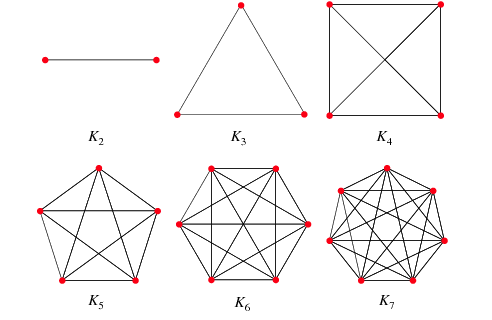
\includegraphics[width=0.35\textwidth]{SomeK}
            \end{figure}

            Ahora es obvio que $K_4$ NO tiene pero $K_5$ si.
        \end{SmallIndentation}


    % ===============================================
    % ========              12                 =======
    % ===============================================
    \section{Pregunta 12}

        % ======== DEMOSTRACION ========
        \begin{SmallIndentation}[1em]
            \textbf{Demostración}:
        
            Es seguir la idea $K_n$ tiene un circuito euleriano si es todos sus vértices tiene grado par.
            Por lo tanto $K_n$ tiene un circuito euleriano si $n$ es impar.

        \end{SmallIndentation}


    % ===============================================
    % ========              12                 =======
    % ===============================================
    \section{Pregunta 13}

        % ======== DEMOSTRACION ========
        \begin{SmallIndentation}[1em]
            \textbf{Demostración}:
        
            No, basta modelarla y ver que lo que se nos pide es un circuito euleriano, que no puede existir por el grado impar de muchos vertices.

            \begin{figure}[h]
                \centering
                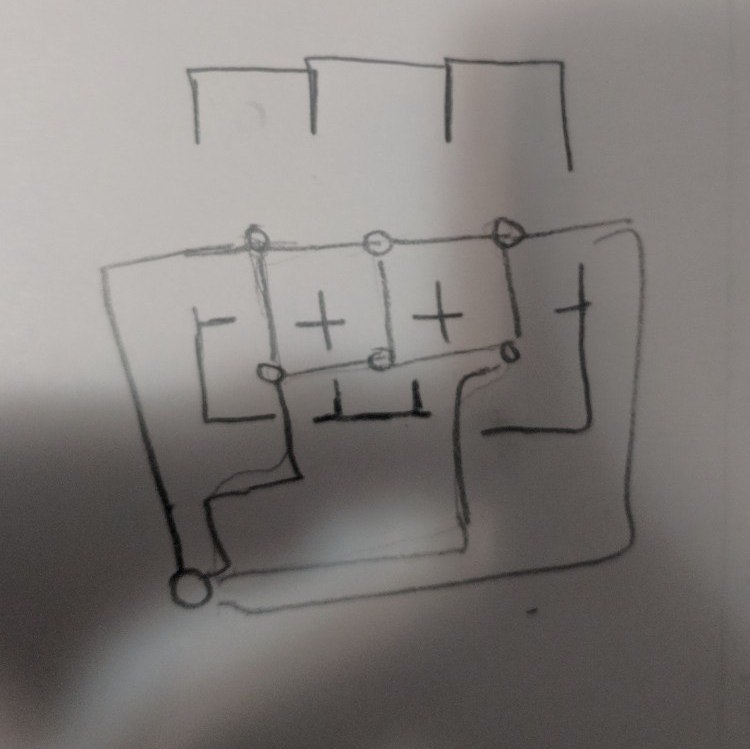
\includegraphics[width=0.35\textwidth]{Question13}
            \end{figure}



        \end{SmallIndentation}

    % ===============================================
    % ========              12                 =======
    % ===============================================
    \section{Pregunta 14}

        % ======== DEMOSTRACION ========
        \begin{SmallIndentation}[1em]
            \textbf{Demostración}:
        
            \begin{figure}[h]
                \centering
                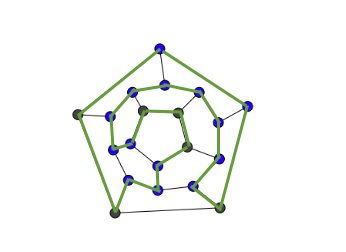
\includegraphics[width=0.55\textwidth]{Question14}
            \end{figure}


        \end{SmallIndentation}


    % ===============================================
    % ========              16                =======
    % ===============================================
    \section{Pregunta 16}

        % ======== DEMOSTRACION ========
        \begin{SmallIndentation}[1em]
            \textbf{Demostración}:


            Queremos probar que $2 |E| = \sum_{v \in V} deg(v)$ para graficas simple, es decir sin loops.

            Sea $n$ el número de aristas de nuestro grafo $G(V, E)$.

            La prueba será por inducción sobre el número de aristas:
            \begin{itemize}
                \item El caso base si $n = 0$, pues si no hay aristas entonces es obvio que la suma da cero.
                    y $2 * 0 = 0$ que es el resultado correcto.

                \item Ahora supongamos cierto para una $n$ cualquiera
                
                \item Ahora si tuviera un grafo con $n+1$ aristas entonces tenemos que podemos pensar así:
                
                Si quitamos un arista entonces volvemos a tener un grafo $G'(V', E')$ que por la hipotesis de inducción
                tiene que pasar que $2n = \sum_{v \in V'} deg(v)$ ahora si añado de regreso la arista vamos a añadir
                1 al grado de 2 vértices es decir: 
                $2n + 2 = \sum_{v \in V} deg(v) = 2(n+1)$, que es justo lo que queríamos.
            \end{itemize}
        
        \end{SmallIndentation}



    % ===============================================
    % ========              15                =======
    % ===============================================
    \clearpage
    \section{Pregunta 15}

    Un grafo tiene un circuito euleriano si y solo si es que todos sus vértices tienen grado par y es conexo

    % ======== DEMOSTRACION ========
    \begin{SmallIndentation}[1em]
        \textbf{Demostración}:
    
        Un circuito euleriano es un recorrido de todas las aristas de un gráfico simple
        una y solo una vez, iniciando en un vértice y terminando en el mismo vértice.
        
        Se puede repetir los vértices tantas veces como queramos, pero nunca se puede repetir
        una arista una vez que la recorremos.

        El grado de un vértice es el número de aristas que inciden en este vértice.

        Entonces, sea G una gráfica que tenga un circuito euleriano. 
        Cada vez que llegamos a un vértice durante nuestro recorrido de G, 
        entramos por una arista y salimos por otra.
        
        Por lo tanto, debe haber un número par de aristas incidentes en cada vértice.
        Por lo tanto, cada vértice de G tiene grado par.

        Siendo más formales:
        \begin{itemize}
            \item Supongamos primero que tenemos una gráfica con un circuito euleriano
                que va como $v_0, v_1, \dots, v_k$ donde $v_0 = v_k$.

                Ya que pasamos por cada arista una vez entonces la longitud de circuito
                es a cantidad de aristas.

                Ahora podemos definir de otra manera el grado de un nodo como la cantidad
                de veces que aparecen en la secuencia $v_0, v_1, \dots, v_{k-1}$ multiplicado
                por dos, multiplicamos por dos porque si $u = v_i$ entonces $v_{i-1}, v_i$
                y $v_{i}, v_{i+1}$ son aristas que inciden en el nodo $u$. 
                Y si $u = v_0$ entonces $v_{k-1}, v_k$ y $v_{0}, v_{1}$ son aristas que inciden
                sobre $v_0$. Por lo tanto todos los vértices tienen grado par.

            \item
                Ahora hay que ver porque es que si el grado de cada nodo es par y el grafo es conexo entonces
                tiene que existir un circuito euleriano si o si.

                Para hacerlo definimos a $W := v_0, v_1, \dots, v_{k}$ com el camino mas grande en nuestro grafo que no
                pasa por mas una arista mas de una vez.

                Ahora, sabemos que $W$ tiene que pasar por cada una de las aristas
                que llegan a $v_k$ sino podriamos extender a $W$ para que sea mas grande.
                
                Ahora, tiene que pasar que $v_0 = v_k$ y por lo tanto que $W$ es un circuito
                porque sino entonces $v_k$ tendría un grado impar. Ahora podría ir por contradicción 
                y decir que $W$ no es euleriano porque no pasa por todas las aristas
                (como G es conexo tenemos que podemos siempre encontrar una arista que no esta en $W$
                pero si que incide a un vértice que esta en $W$), llamemoslo $(u, v_i)$, pero, entonces
                sería muy fácil extender a una $W'$ que si que lo hiciera como: 
                $W' = u, v_i, v_{i+1}, \dots, v_k, v_1, v_2, \dots, v_i$.

                Por lo tanto $W$ tiene que ser un circuto euleriano.

        \end{itemize}

    \end{SmallIndentation}



    


    % ===============================================
    % ========              17                =======
    % ===============================================
    \clearpage
    \section{Pregunta 17}

        Demostrar que si G es bipartita entonces todos los ciclos que contiene G
        tienen una cantidad par de vértices

        % ======== DEMOSTRACION ========
        \begin{SmallIndentation}[1em]
            \textbf{Demostración}:
                Una dirección es un sencilla:
                Si es que G es bipartito con dos conjuntos $V_1$, $V_2$, entonces cada paso a lo largo de un ciclo te manda o bien de 
                $V_1$ a $V_2$ o de $V_2$ a $V_1$, para acabar donde empezaste, por lo tanto tienes que tomar un numero par de pasos.

                Por otro lado, suponte que cada ciclo dentro de nuestro grafo tiene una longitud par, para cada vértice $v_0$ en el
                mismo componente $C_0$ que $v_0$, sea $d(v)$ sea la longitud del camino más corto de $v_0$ a $v$.
                
                Colorea de rojo cada vértice en $C_0$ cuya distancia desde $v_0$ sea par, y colorea los otros vértices de $C_0$de azul. 
                Hacemos lo mismo para cada componente del grafo, ahora ve que si nuestro grafo tuviera una arista entre dos
                vértices rojos o entre dos vértices azules, tendríamos un ciclo impar.
                
                Por lo tanto, G es bipartito, con los vértices rojos y azules siendo las dos partes.
            
        \end{SmallIndentation}


    % ===============================================
    % ========              17                =======
    % ===============================================
    \clearpage
    \section{Pregunta 18}

        Demostrar que la cantidad de vértices de grado impar de una grafo G es
        par

        % ======== DEMOSTRACION ========
        \begin{SmallIndentation}[1em]
            \textbf{Demostración}:

                La suma de todos los grados es igual al doble del número de aristas.
                Dado que la suma de los grados es par y ya que vamos a separar a las suma en otras 2 sumas, amabas tienen que ser o impar o par.
                Pero sabemos que la suma de los grados de los vértices con grado par es par, así que 
                la suma de los grados de vértices con grado impar debe ser par.
                
                Si la suma de los grados de vértices con grado impar es par, debe haber un número par de esos vértices, pues solo sumando
                una cantidad par de números impares obtenemos par.
            
        \end{SmallIndentation}

    % ===============================================
    % ========              19                =======
    % ===============================================
    \clearpage
    \section{Pregunta 19}

        Demostrar que el máximo número de aristas en una grafo G es $\dfrac{n(n-1)}{2}$ con $n$ numero de vertices 

        % ======== DEMOSTRACION ========
        \begin{SmallIndentation}[1em]
            \textbf{Demostración}:

                Una idea sencilla, el grafo que mas aristas podría tener dejando fijo en numero de vertices sería un grafo completo,
                es decir que cada vértice está conectado con cada otro vértice.
                Si tomamos un vértice, por lo tanto tiene $n-1$ aristas saliendo de el.

                Ahora, si tenemos n vértices en total, sería lógico pensar que hay $n (n- 1)$ aristas en total.
                Pero este método cuenta cada arista dos veces, porque cada arista que sale de un vértice es una arista que va a otro vértice.
                Por lo tanto, hay que dividir entre dos, dejandonos con: $\dfrac{n(n-1)}{2}$
        \end{SmallIndentation}


    % ===============================================
    % ========              21                =======
    % ===============================================
    \clearpage
    \section{Pregunta 21}

        Construye una gráfica bipartita hamiltoniana y no euleriana.

        Este esta sencillo, no puede ser Euleriano porque todos sus vertices tienen grado impar, pero el camino hamiltoniano es super sencillo
        es simplemente caminar por la parte exterior.

                
        \begin{figure}[h]
            \centering
            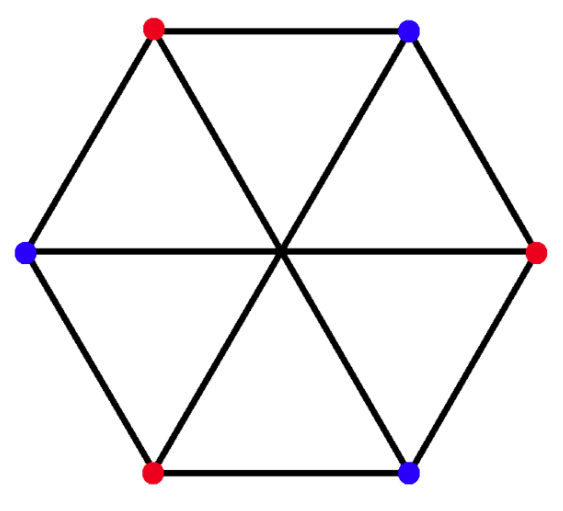
\includegraphics[width=0.55\textwidth]{Question21}
        \end{figure}



    % ===============================================
    % ========              23                =======
    % ===============================================
    \clearpage
    \section{Pregunta 23}

   
        Proporcione una gráfica que contenga ciclo eulerino y no tenga ciclo hamiltonino, y una con ciclo hamiltoniano pero no tenga ciclo euleriano
                
        \begin{figure}[h]
            \centering
            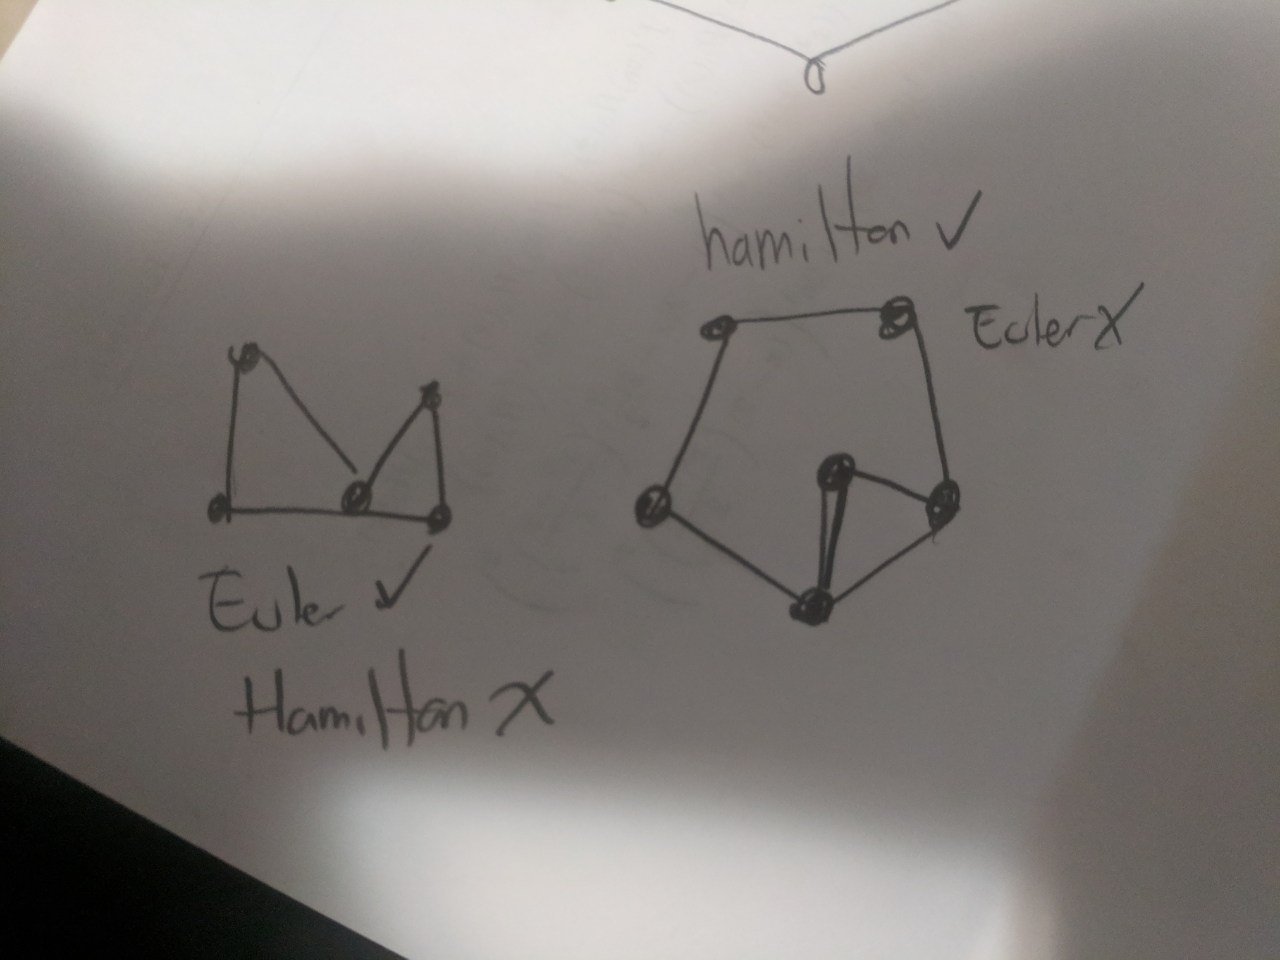
\includegraphics[width=0.55\textwidth]{Question23}
        \end{figure}


    % ===============================================
    % ========              24                =======
    % ===============================================
    \clearpage
    \section{Pregunta 24}

   
        De una gráfica que contenga un ciclo euleriano que también sea un ciclo
        hamiltoniano y otra donde sean distintos

        \begin{figure}[h]
            \centering
            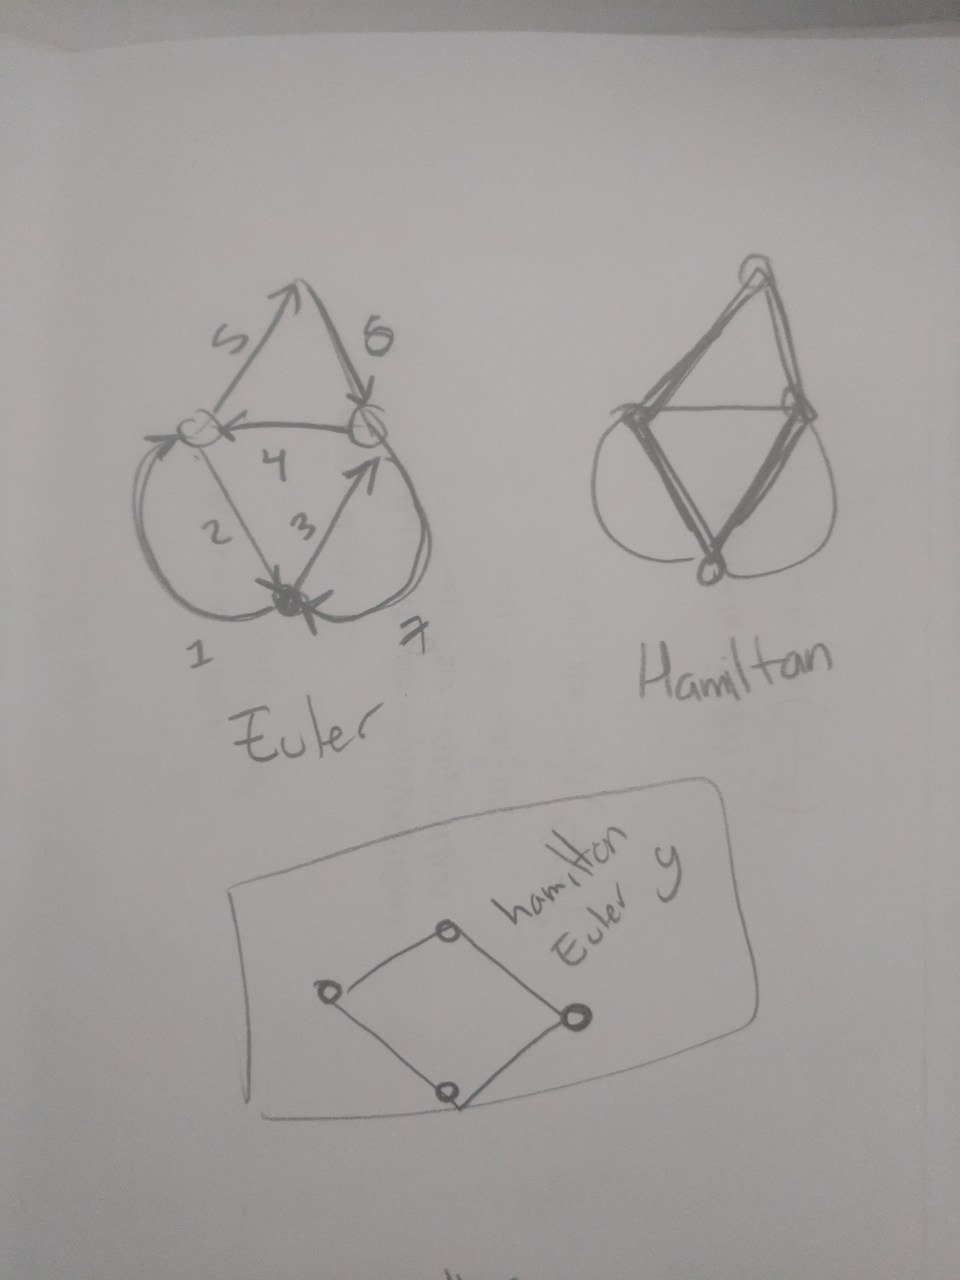
\includegraphics[width=0.55\textwidth]{Question24}
        \end{figure}



    % ===============================================
    % ========              25                =======
    % ===============================================
    \section{Pregunta 25}

        Muestra que si n > 2 la gráfica completa de n vértices Kn tiene un ciclo
        hamiltoniano

        % ======== DEMOSTRACION ========
        \begin{SmallIndentation}[1em]
            \textbf{Demostración}:
        
            Llamemos a los vertices $v_1, v_2, \dots, v_n$ entonces si empezamos el ciclo en $v_1$ como nuestro grafo es 
            $k_n$ es completo por lo que estamos seguros de que existe una arista a $v_2$ de ahi tomamos la arista que seguro
            tambien tiene que existir y así hasta que estemos en $v_n$ de ahi de nuevo porque nuestro grafo es completo podemos
            asegurar de que existe una arista de regreso a $v_1$ con eso cerrando el ciclo.
        
        \end{SmallIndentation}

    % ===============================================
    % ========              26                =======
    % ===============================================
    \section{Pregunta 26}


       Este estuvo buena, tuve que programar Dijkstra, pero fue mas rapido que andar haciendo las cuentas a mano
       les dejo el codigo asi como ss del resultado, eso si, por coherencia cambie la $x$ por una $a$ para que todo quede bonito.

        \lstinputlisting[language=C++, gobble=8]{Dijkstra.cpp}

        Y la entrada que presenta el grafo, la primera linea es el numero de nodos, de aristas y el nodo origen,
        despues son una lista de 3 elementos que representan aristas, que es inicio, final y peso.

        \lstinputlisting[language=C++, gobble=8]{Input26.in}

        \begin{figure}[h]
            \centering
            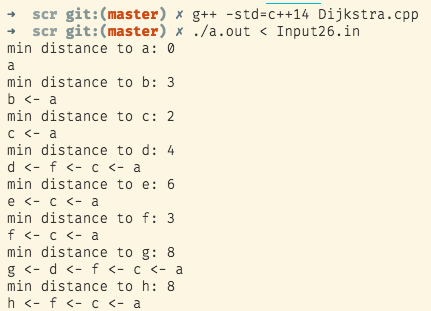
\includegraphics[width=0.55\textwidth]{Question26}
        \end{figure}


    % ===============================================
    % ========              27                =======
    % ===============================================
    \clearpage
    \section{Pregunta 27}

        Aqui el input que usamos:
        \lstinputlisting[language=C++, gobble=8]{Input27.in}

        \begin{figure}[h]
            \centering
            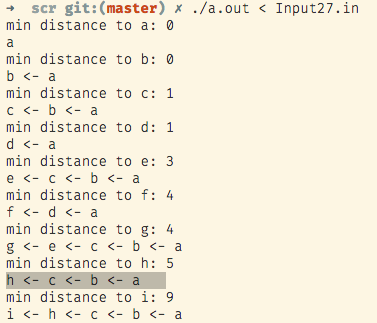
\includegraphics[width=0.55\textwidth]{Question27}
        \end{figure}




                
\end{document}